\documentclass[a4paper,doc,floatsintext,natbib,10pt]{article}
% \shorttitle{Flow Experience and Spontaneous Blink Rate -- Supplementary Information}

% insert here the call for the packages your document requires
\usepackage{graphics}
\graphicspath{{./Figures/}}
\usepackage{amsmath}
\usepackage{amsfonts}
\usepackage{amssymb}
\usepackage{url}
\usepackage{xspace}
\usepackage{textcomp}
\usepackage{xcolor}
\usepackage{varwidth}
\usepackage{caption}
\usepackage[normalem]{ulem}

\begin{document}

\subsection*{Flow Short Scale, in English with Finnish Translation}

\begin{minipage}{\textwidth}
\begin{tabular}{l p{0.4\textwidth} p{0.4\textwidth}}
\multicolumn{3}{l}{Core items of Flow: {\it fluency of performance} (2, 4, 5, 7, 8, 9) and {\it absorption by activity} (1, 3, 6, 10):} \\
\\
1. & I feel just the right amount of challenge    &    Peli tuntui juuri sopivan haastavalta  \\
2. & My thoughts/activities run fluidly and smoothly   & Pelasin sujuvasti \\
3. & I do not notice time passing  & En huomannut ajankulkua \\
4. & I have no difficulty concentrating & Pystyin hyvin keskittym\"{a}\"{a}n \\
5. & My mind is completely clear & Mieleni oli selke\"{a} \\
6. & I am totally absorbed in what I am doing & Uppouduin t\"{a}ysin pelaamiseen \\
7. & The right thoughts/movements occur of their own accord & L\"{o}ysin oikeat liikkeet kuin itsest\"{a}\"{a}n \\
8. & I know what I have to do each step of the way & Olin koko ajan tilanteen tasalla \\
9. & I feel that I have everything under control & Tunsin hallitsevani tilannetta \\
10. & I am completely lost in thought & Syvennyin peliin t\"{a}ysin  \\
\\
\multicolumn{3}{l}{Extra items for {\it perceived importance}:} \\
\\
11. & Something important to me is at stake here & Koin peliss\"{a} onnistumisen t\"{a}rke\"{a}ksi \\
12. & I must not make any mistakes here & Minusta tuntui silt\"{a}, etten saisi tehd\"{a} yht\"{a}k\"{a}\"{a}n virhett\"{a}\\
13. & I am worried about failing & Pelk\"{a}sin ep\"{a}onnistuvani\\
\\
\multicolumn{3}{l}{Extra items for the fit of skills and demands:} \\
\\
14. & Compared to all other activities which I partake in,this one is... (easy/difficult) & Verrattuna muihin tekemiini asioihin, t\"{a}m\"{a} on... (helppoa/vaikeaa) \\
15. & I think that my competence in this area is... (low/high)  & Osaamiseni taso on... (matala/korkea)\\
16. & For me personally, the current demands are... (too low/just right/too high) & Pelin vaativuus on t\"{a}ll\"{a} hetkell\"{a} minulle... (liian matala/sopiva/liian korkea)\\
\end{tabular}
\end{minipage}

\begin{table}[!h]
\centering
\caption{\label{tab:FluencyAbsorption}Descriptive statistics for fluency of performance and absorption by activity for each participant.}
\begin{tabular}{lllllll}
\hline
           & Participant & Mean & Median & SD   & Min  & Max  \\
\hline
Fluency    &             &      &        &      &      &      \\
           & 1           & 4.93 & 5.00   & .62  & 3.17 & 6.00 \\
           & 2           & 4.90 & 4.83   & .47  & 3.83 & 5.67 \\
           & 3           & 4.90 & 5.00   & .84  & 3.00 & 6.67 \\
           & 4           & 4.10 & 4.00   & .56  & 3.00 & 5.33 \\
           & 5           & 5.15 & 5.50   & 1.01 & 2.67 & 6.50 \\
           & 6           & 5.11 & 5.25   & .92  & 2.83 & 6.50 \\
           & 7           & 4.35 & 4.33   & .58  & 3.17 & 5.50 \\
           & 8           & 4.74 & 5.00   & .92  & 2.50 & 6.33 \\
           & 9           & 5.24 & 5.00   & .86  & 3.33 & 7.00 \\
\hline
Absorption &             &      &        &      &      &      \\
           & 1           & 5.37 & 5.50   & .45  & 4.25 & 6.25 \\
           & 2           & 5.60 & 5.75   & .37  & 5.00 & 6.00 \\
           & 3           & 6.04 & 6.00   & .43  & 5.25 & 6.75 \\
           & 4           & 4.85 & 4.88   & .39  & 4.00 & 5.75 \\
           & 5           & 5.89 & 6.0    & .80  & 3.50 & 7.00 \\
           & 6           & 5.37 & 5.50   & .74  & 3.50 & 6.75 \\
           & 7           & 5.19 & 5.25   & .54  & 4.25 & 6.25 \\
           & 8           & 5.24 & 5.50   & .95  & 3.00 & 6.75 \\
           & 9           & 5.27 & 5.13   & .72  & 4.00 & 6.75 \\
\hline
\end{tabular}
\end{table}

\noindent
\begin{minipage}{\textwidth}
\centering
% 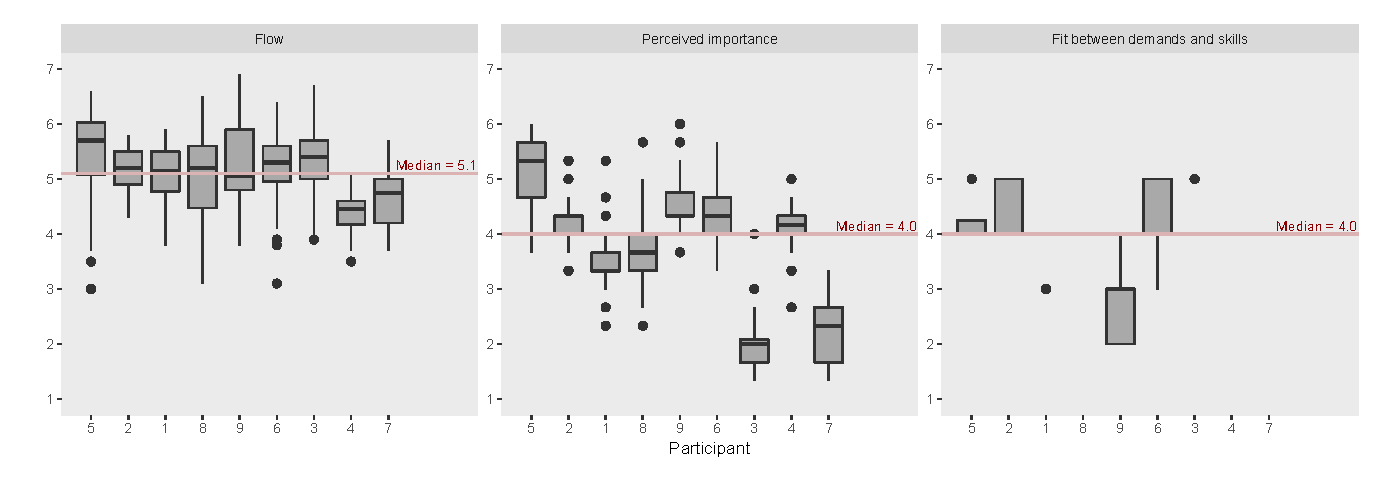
\includegraphics[width=\linewidth]{suppl_fss_boxplots}
\captionof{figure}{Participant-wise boxplots for Flow Short Scale measures, {\it left panel}: Flow (absorption \& fluency), median 5.1, min 3, max 7; {\it center panel}: perceived importance, median 4, min 1, max 6; {\it right panel}: perceived fit of demands and skills, median 4, min 2, max 5. In each plot, boxes are ordered left-to-right by the game performance (mean trial duration) of participants, i.e. from best performer \#5 to worst \#7.}
\label{fig:supp_boxes}
\end{minipage}

%%%%%%%%%%%%%%% END OF SUPPLEMENTARY %%%%%%%%%%%%%%%
\end{document}
